% =====================================================================
%  Mathematical derivations -- stability of the shared-control loop
%  Pragyan Mohanty, roll 24250
%
%  Compile from this folder (report/):
%      pdflatex math_derivation.tex
%      pdflatex math_derivation.tex
% =====================================================================
\documentclass[11pt,a4paper]{article}

\usepackage[T1]{fontenc}
\usepackage[utf8]{inputenc}
\usepackage{lmodern}
\usepackage{microtype}
\usepackage[margin=2.3cm]{geometry}
\usepackage{amsmath,amssymb,amsthm}
\usepackage{mathtools}
\usepackage{cancel}
\usepackage{graphicx}
\usepackage{booktabs}
\usepackage{caption}
\usepackage{float}
\usepackage{xcolor}
\usepackage[colorlinks=true,linkcolor=black,citecolor=black,urlcolor=blue]{hyperref}

\graphicspath{{../results/part2/figures/}}
\captionsetup{font=small,labelfont=bf,justification=raggedright,singlelinecheck=true}
\setlength{\parindent}{0pt}
\setlength{\parskip}{0.5em}
\setlength{\emergencystretch}{2em}

\newcommand{\ptwo}[1]{{\small\textsf{[P2~\S#1]}}}
\newcommand{\code}[1]{\texttt{#1}}
\newtheorem{result}{Result}
\theoremstyle{definition}
\newtheorem*{idea}{Key idea}

\begin{document}

% ---------------------------------------------------------------------
\begin{center}
{\LARGE\bfseries Stability of a Shared-Control Loop under Delay}\\[0.5em]
{\large Mathematical derivations}\\[0.9em]
Pragyan Mohanty \quad (Roll No.\ 24250)\\[0.2em]
Control Systems course project
\end{center}
\vspace{0.5em}

% =====================================================================
\section{Introduction}

\textbf{Context.} In this project a wheelchair is driven by two
controllers at once. The \emph{user} steers through an EEG decoder; an
\emph{autopilot} plans safe motion on its own. Their commands are mixed
as
\begin{equation}
u = \alpha\,u_{\mathrm{user}} + (1-\alpha)\,u_{\mathrm{auto}},
\qquad \alpha \in [0,1],
\label{eq:blend}
\end{equation}
where $\alpha$ is the user's share of control. The user's path is
\emph{delayed}: the user reacts late, and the decoder needs time to
decide. The autopilot's path is not delayed.

\textbf{Why delay matters.} A feedback controller corrects the error it
sees. If what it sees is old, it keeps pushing after the error has
already been corrected, overshoots, and then corrects the overshoot
late as well. A small delay only makes the response less damped; a large
enough delay makes each overshoot bigger than the last, and the loop
oscillates without bound. That is instability.

\textbf{The question.} The more weight $\alpha$ the delayed user gets,
the more the loop depends on old information. So we ask:
\begin{center}
\emph{For each share $\alpha$, what is the largest loop delay
$\tau_{\max}(\alpha)$ that keeps the closed loop stable?}
\end{center}

\textbf{Outline.}
Section~\ref{sec:model} sets up the model and explains why the
derivation uses a simpler plant than the simulation.
Section~\ref{sec:lqr} derives the autopilot's LQR gains.
Section~\ref{sec:char} forms the characteristic equation and explains
why the usual tools cannot be applied to it.
Sections~\ref{sec:crossing}--\ref{sec:taumax} derive $\tau_{\max}(\alpha)$
exactly. Section~\ref{sec:alphastar} finds the range of $\alpha$ that is
stable for every delay. Section~\ref{sec:heading} applies the method to
the wheelchair's heading loop. Section~\ref{sec:checks} checks the result
numerically, and Section~\ref{sec:limits} states the limitations and
future work.

The numerical results quoted here are produced by Section~7 of the Part~2
notebook (\code{src/part2\_shared\_control.ipynb}); references of the
form \ptwo{7.2} point to the relevant notebook section. The results are
summarised in the main report, \code{report.pdf}, Section~6.

% =====================================================================
\section{The model}
\label{sec:model}

\subsection{Two models, two purposes}

\textbf{The simulation uses the wheelchair model.} All wheelchair
experiments in the project use a \emph{unicycle} model: position
$(x,y)$, heading $\theta$, forward speed $v$ and turn rate $\omega$,
with motor lags, speed and acceleration limits, and the constraint that
the chair cannot move sideways (Section~\ref{sec:heading} gives its
equations). This model is nonlinear: the position depends on
$\cos\theta$ and $\sin\theta$, and the limits clip the inputs.

\textbf{The derivation uses a double integrator.} A nonlinear model with
saturations has no closed-form delay boundary. To obtain an \emph{exact}
answer we analyse a simpler linear plant: one axis of a point mass with
damping. It keeps the features that matter for the question (a delayed
and an undelayed controller acting on the same second-order plant) and
drops the rest. Section~\ref{sec:heading} then carries the same method
back to the wheelchair's turning loop, and states what that step
leaves out.

\subsection{The double-integrator plant}

One axis of a point mass with velocity damping $d$:
\begin{equation}
\dot p = v, \qquad \dot v = u - d\,v ,
\qquad\text{i.e.}\qquad
\dot x = A x + B u,\quad
x = \begin{bmatrix} p\\ v\end{bmatrix},\;
A = \begin{bmatrix} 0 & 1\\ 0 & -d\end{bmatrix},\;
B = \begin{bmatrix} 0\\ 1\end{bmatrix},
\label{eq:plant}
\end{equation}
with $d = 1$. The input $u$ is an acceleration command; the damping term
$-d\,v$ makes the mass slow down by itself when no input is applied.

\textbf{Error coordinates.} Let $g$ be the goal position and
$z = p - g$ the position error. Since $g$ is constant, $\dot z = v$ and
$\ddot z = u - d\,\dot z$. Reaching the goal means driving $z$ to zero,
so from now on everything is written in terms of $z$.

\subsection{The two controllers}

\textbf{The user} is modelled as a proportional--derivative (PD)
controller that sees the state $\tau$ seconds late:
\begin{equation}
u_{\mathrm{user}}(t) = -K_p\,z(t-\tau) - K_d\,\dot z(t-\tau),
\qquad K_p = 4,\; K_d = 2 .
\label{eq:user}
\end{equation}
The P term pushes toward the goal, harder when the error is larger; the
D term brakes against the speed already built up. In the analysis
$\tau$ stands for the \emph{total} delay around the user's path, not
only the user's own 0.2\,s reaction time.

\textbf{The autopilot} is a state-feedback controller with no delay,
\begin{equation}
u_{\mathrm{auto}}(t) = -K_1\,z(t) - K_2\,\dot z(t),
\label{eq:auto}
\end{equation}
with gains $K_1, K_2$ chosen by LQR (next section). In the simulation
the autopilot is a planner (the Dynamic Window Approach), not an LQR
controller; LQR is its linear stand-in for this analysis.

% =====================================================================
\section{The autopilot gains: LQR}
\label{sec:lqr}

\subsection{The idea}
The \emph{linear--quadratic regulator} chooses the feedback $u = -Kx$
that minimises
\begin{equation}
J = \int_0^\infty \bigl( x^{\!\top} Q\, x + u^{\!\top} R\, u \bigr)\,dt
  = \int_0^\infty \bigl( q_p\, z^2 + q_v\, \dot z^2 + r\, u^2 \bigr)\,dt ,
\qquad Q = \begin{bmatrix} q_p & 0\\ 0 & q_v\end{bmatrix},\; R = r,
\end{equation}
with $q_p = 10$, $q_v = 1$, $r = 1$. The first two terms penalise being
far from the goal and moving fast; the last penalises control effort.
The ratio of the weights sets the trade-off: a larger $q_p/r$ gives a
more aggressive controller.

For a linear plant and a quadratic cost, the optimal law is linear,
\begin{equation}
K = R^{-1}B^{\!\top}P,
\label{eq:kformula}
\end{equation}
where $P$ is the symmetric, positive-definite solution of the
\emph{algebraic Riccati equation} (ARE)
\begin{equation}
A^{\!\top} P + P A - P B R^{-1} B^{\!\top} P + Q = 0 .
\label{eq:are}
\end{equation}
The minimum cost from a starting state $x_0$ is $x_0^{\!\top} P x_0$,
which is why $P$ must be positive definite: the cost of any non-zero
starting error is positive.

\subsection{Solving the Riccati equation by hand}

Write the unknown symmetric matrix as
$P = \begin{bmatrix} p_{11} & p_{12}\\ p_{12} & p_{22}\end{bmatrix}$
and compute each term of \eqref{eq:are} in turn.

\textbf{Term 1 and 2.}
\[
PA = \begin{bmatrix} p_{11} & p_{12}\\ p_{12} & p_{22}\end{bmatrix}
     \begin{bmatrix} 0 & 1\\ 0 & -d\end{bmatrix}
   = \begin{bmatrix} 0 & p_{11} - d\,p_{12}\\ 0 & p_{12} - d\,p_{22}\end{bmatrix},
\qquad
A^{\!\top}P = (PA)^{\!\top}
   = \begin{bmatrix} 0 & 0\\ p_{11} - d\,p_{12} & p_{12} - d\,p_{22}\end{bmatrix}.
\]
(The second follows because $P$ is symmetric, so
$A^{\!\top}P = A^{\!\top}P^{\!\top} = (PA)^{\!\top}$.) Adding them:
\[
A^{\!\top}P + PA =
\begin{bmatrix} 0 & p_{11} - d\,p_{12}\\ p_{11} - d\,p_{12} & 2p_{12} - 2d\,p_{22}\end{bmatrix}.
\]

\textbf{Term 3.} Since $B = [0\;\,1]^{\!\top}$ picks out the second
column of $P$,
\[
PB = \begin{bmatrix} p_{12}\\ p_{22}\end{bmatrix},
\qquad
PBR^{-1}B^{\!\top}P = \frac{1}{r}\begin{bmatrix} p_{12}\\ p_{22}\end{bmatrix}
\begin{bmatrix} p_{12} & p_{22}\end{bmatrix}
= \frac{1}{r}\begin{bmatrix} p_{12}^2 & p_{12}p_{22}\\ p_{12}p_{22} & p_{22}^2\end{bmatrix}.
\]

\textbf{Putting the ARE together.} Adding $Q$ and subtracting term 3,
\[
\begin{bmatrix}
q_p - p_{12}^2/r & \; p_{11} - d\,p_{12} - p_{12}p_{22}/r\\[2pt]
p_{11} - d\,p_{12} - p_{12}p_{22}/r & \; 2p_{12} - 2d\,p_{22} - p_{22}^2/r + q_v
\end{bmatrix}
= \begin{bmatrix} 0 & 0\\ 0 & 0\end{bmatrix}.
\]
The matrix is symmetric, so it gives three distinct scalar equations:
\begin{align}
(1,1):&\quad q_p - p_{12}^2/r = 0, \label{eq:r11}\\
(1,2):&\quad p_{11} - d\,p_{12} - p_{12}\,p_{22}/r = 0, \label{eq:r12}\\
(2,2):&\quad 2p_{12} - 2d\,p_{22} - p_{22}^2/r + q_v = 0. \label{eq:r22}
\end{align}

\textbf{Solving in order.}
\begin{enumerate}\setlength{\itemsep}{2pt}
\item From \eqref{eq:r11}, $p_{12}^2 = r\,q_p$, so
$p_{12} = \pm\sqrt{r\,q_p}$. We take the positive root: with the
negative one, \eqref{eq:r22} becomes $p_{22}^2 + 2p_{22} + 5.32 = 0$,
which has no real solution. Hence $p_{12} = \sqrt{10} = 3.162278$.
\item Equation \eqref{eq:r22} now contains only $p_{22}$. Multiplying by
$-r$ gives a quadratic,
\[
p_{22}^2 + 2rd\,p_{22} - r\,(q_v + 2p_{12}) = 0
\;\Rightarrow\;
p_{22} = -rd \pm \sqrt{r^2d^2 + r\,(q_v + 2p_{12})}.
\]
A positive-definite $P$ needs $p_{22} > 0$, so we take the $+$ sign:
$p_{22} = -1 + \sqrt{1 + 1 + 2\sqrt{10}} = -1 + 2.885231 = 1.885231$.
\item Equation \eqref{eq:r12} then gives
$p_{11} = d\,p_{12} + p_{12}p_{22}/r = 9.123900$. The gain does not use
$p_{11}$, but it completes $P$, and one can check that $P$ is positive
definite ($p_{11} > 0$ and $p_{11}p_{22} - p_{12}^2 = 7.20 > 0$).
\end{enumerate}

\textbf{The gains.} From \eqref{eq:kformula},
$K = R^{-1}B^{\!\top}P = \frac{1}{r}\,[0\;\,1]\,P = [p_{12}\;\,p_{22}]/r$:
\begin{equation}
\boxed{\;K_1 = \sqrt{\frac{q_p}{r}} = 3.162278,
\qquad
K_2 = -d + \sqrt{d^2 + \frac{q_v + 2\sqrt{r q_p}}{r}} = 1.885231\;}
\label{eq:lqr}
\end{equation}
The notebook obtains the same numbers from this formula and from a
numerical Riccati solver \ptwo{3.2}.

\textbf{Check: the autopilot alone is stable.} With $\alpha = 0$ the loop
is $\ddot z + (d + K_2)\dot z + K_1 z = 0$, with characteristic
polynomial $s^2 + 2.885231\,s + 3.162278$. Its roots are
$s = -1.443 \pm 1.040j$: both have negative real parts, with damping
ratio $\zeta = 2.885231/(2\sqrt{3.162278}) = 0.81$, so the autopilot
alone brings the error to zero smoothly with little overshoot.

% =====================================================================
\section{The characteristic equation}
\label{sec:char}

\subsection{The closed loop with delay}
Substituting \eqref{eq:user} and \eqref{eq:auto} into the plant with
shares $\alpha$ and $1-\alpha$ gives
\begin{equation}
\ddot z + d\,\dot z
+ (1-\alpha)\bigl(K_1 z + K_2 \dot z\bigr)
+ \alpha\bigl(K_p\, z(t-\tau) + K_d\, \dot z(t-\tau)\bigr) = 0 .
\label{eq:dde}
\end{equation}
This is a \emph{delay differential equation} (DDE): its right-hand side
uses past values of $z$ as well as current ones.

\subsection{From the DDE to roots}
\textbf{What roots mean.} As for an ordinary linear ODE, we look for
solutions of the form $z(t) = e^{st}$. Writing $s = \sigma + j\omega$,
\[
e^{st} = e^{\sigma t}\bigl(\cos\omega t + j\sin\omega t\bigr):
\]
an oscillation at frequency $\omega$ whose size is multiplied by
$e^{\sigma t}$. If $\sigma < 0$ the oscillation dies out; if
$\sigma > 0$ it grows without bound. The general response is a sum of
such terms, one per root (pole), so the loop is \textbf{stable exactly
when every root has negative real part}, i.e.\ lies in the left half of
the complex plane. A root \emph{on} the imaginary axis ($\sigma = 0$)
gives an oscillation that neither grows nor decays: the edge of
stability.

\textbf{The equation.} Substituting $z = e^{st}$, a delayed term becomes
$z(t-\tau) = e^{s(t-\tau)} = e^{-\tau s}e^{st}$, i.e.\ the delay
multiplies by $e^{-\tau s}$ (the same rule as
$\mathcal{L}\{z(t-\tau)\} = e^{-\tau s}Z(s)$ in the Laplace domain).
Dividing through by $e^{st}$:
\begin{equation}
\boxed{\;\Delta(s) = \underbrace{s^{2} + d\,s + (1-\alpha)(K_1 + K_2 s)}_{\mathcal{P}(s)\ \text{(undelayed)}}
+ \underbrace{\alpha (K_p + K_d s)}_{\mathcal{Q}(s)\ \text{(delayed)}}\,e^{-\tau s} = 0 \;}
\label{eq:char}
\end{equation}
$\mathcal{P}(s)$ collects the plant and the autopilot; $\mathcal{Q}(s)$
is the user's part, which is the only part multiplied by the delay.

\subsection{Why the usual tools do not work}
For a loop without delay, $\Delta(s)$ is a polynomial, and the standard
tools apply. Here they do not:
\begin{itemize}\setlength{\itemsep}{2pt}
\item \textbf{Routh--Hurwitz} decides stability from the coefficients of
a polynomial of finite degree. But
$e^{-\tau s} = 1 - \tau s + \tfrac{(\tau s)^2}{2!} - \dots$ is an
infinite series, so $\Delta(s)$ is not a polynomial; it is a
\emph{quasi-polynomial} with infinitely many coefficients and
\emph{infinitely many roots}. There is no finite Routh table to build.
\item \textbf{Root locus} plots how the roots of a \emph{fixed}
polynomial move as a \emph{gain} multiplying part of it is varied. Its
rules (number of branches equals the order, asymptote angles, break-away
points) all rely on a finite order. Here the varying parameter $\tau$
sits inside the exponential rather than multiplying the equation, and
there are infinitely many branches, so the rules do not apply.
\item \textbf{Replacing the delay by an approximation} (for example a
Pad\'e approximation, Section~\ref{sec:checks}) restores a polynomial,
but the answer is then only approximate, and we will see that it errs in
the unsafe direction.
\end{itemize}

\subsection{The way around it}
We do not need all the roots: we only need the delay at which the
\emph{first} root becomes unstable. Two facts make this tractable.
\begin{enumerate}\setlength{\itemsep}{2pt}
\item \textbf{With no delay the loop is stable.} At $\tau = 0$,
$\Delta(s) = s^2 + \bigl(d + (1-\alpha)K_2 + \alpha K_d\bigr)s
+ \bigl((1-\alpha)K_1 + \alpha K_p\bigr)$. For a second-order
polynomial, both coefficients positive is necessary and sufficient for
both roots to lie in the left half-plane, and both are positive for
every $\alpha \in [0,1]$.
\item \textbf{Roots move continuously with $\tau$.} As $\tau$ increases
from zero, each root moves along a continuous path. To get from the left
half-plane to the right half-plane it must pass through the boundary
between them, the imaginary axis, at some point $s = j\omega$.
\end{enumerate}
So the loop stays stable as $\tau$ grows \emph{until} the first root
touches the imaginary axis. The plan is therefore: find every
$(\omega, \tau)$ at which $\Delta(j\omega) = 0$, and take the smallest
such $\tau$ at which a root crosses into the right half-plane.

\textbf{Why increasing the delay is what causes the crossing.} At
$s = j\omega$, $|e^{-j\omega\tau}| = 1$ and
$\arg e^{-j\omega\tau} = -\omega\tau$. The delay therefore never changes
the \emph{size} of the user's term; it only adds a phase lag
$\omega\tau$, which grows as $\tau$ grows. A larger lag means the user's
correction arrives later relative to the oscillation it is meant to
damp. When the lag is large enough, the correction arrives in step with
the oscillation and reinforces it instead of opposing it, and a root
reaches the imaginary axis. The derivation below finds exactly when this
happens.

% =====================================================================
\section{Where a root can cross the imaginary axis}
\label{sec:crossing}

\subsection{Setting up}
Substitute $s = j\omega$, with $\omega > 0$, into \eqref{eq:char} and
write $\theta = \omega\tau$ for the phase lag added by the delay. To keep
the algebra short, name the combinations of gains that appear:
\begin{equation}
P_1 = (1-\alpha)K_1,\quad P_2 = d + (1-\alpha)K_2,\quad
Q_1 = \alpha K_p,\quad Q_2 = \alpha K_d ,
\end{equation}
so that $\mathcal{P}(s) = s^2 + P_2 s + P_1$ and
$\mathcal{Q}(s) = Q_2 s + Q_1$. At $s = j\omega$, using $j^2 = -1$:
\begin{equation}
\mathcal{P}(j\omega) = (P_1 - \omega^{2}) + j\,P_2\,\omega = A + jB,
\qquad
\mathcal{Q}(j\omega) = Q_1 + j\,Q_2\,\omega = C + jD,
\end{equation}
where $A = P_1 - \omega^2$, $B = P_2\omega$, $C = Q_1$, $D = Q_2\omega$
are real numbers.

\subsection{Real and imaginary parts}
With $e^{-j\theta} = \cos\theta - j\sin\theta$, the condition
$\Delta(j\omega) = 0$ reads
\[
(A + jB) + (C + jD)(\cos\theta - j\sin\theta) = 0 .
\]
Multiplying out the product,
$(C + jD)(\cos\theta - j\sin\theta) = (C\cos\theta + D\sin\theta)
+ j\,(D\cos\theta - C\sin\theta)$. A complex number is zero only if its
real and imaginary parts are both zero, so
\begin{align}
\text{real part:}&\qquad A + C\cos\theta + D\sin\theta = 0, \label{eq:re}\\
\text{imaginary part:}&\qquad B + D\cos\theta - C\sin\theta = 0. \label{eq:im}
\end{align}
For each $\omega$ these are two equations, and the unknown is the single
angle $\theta$. In general two equations in one unknown have no
solution; they can only be satisfied together at special values of
$\omega$. Finding those values is the next step.

\subsection{Step 1: solve for \texorpdfstring{$\cos\theta$}{cos theta} and \texorpdfstring{$\sin\theta$}{sin theta}}
Treat $\cos\theta$ and $\sin\theta$ as two separate unknowns. Then
\eqref{eq:re}--\eqref{eq:im} are \emph{linear}:
\[
\begin{bmatrix} C & D \\ D & -C \end{bmatrix}
\begin{bmatrix} \cos\theta \\ \sin\theta \end{bmatrix}
=
\begin{bmatrix} -A \\ -B \end{bmatrix},
\qquad \det = -C^2 - D^2 = -(C^2 + D^2) .
\]
The determinant is non-zero whenever $\alpha > 0$ (then $C = \alpha K_p > 0$),
so by Cramer's rule
\begin{equation}
\cos\theta = \frac{\begin{vmatrix} -A & D\\ -B & -C\end{vmatrix}}{-(C^2+D^2)}
           = -\frac{AC + BD}{C^{2}+D^{2}},
\qquad
\sin\theta = \frac{\begin{vmatrix} C & -A\\ D & -B\end{vmatrix}}{-(C^2+D^2)}
           = \frac{BC - AD}{C^{2}+D^{2}}.
\label{eq:cossin}
\end{equation}

\subsection{Step 2: the delay drops out}
The two values in \eqref{eq:cossin} must be the cosine and sine of the
\emph{same} angle, which is only possible if
$\cos^2\theta + \sin^2\theta = 1$. Substituting \eqref{eq:cossin} and
multiplying by $(C^2+D^2)^2$:
\begin{align*}
(AC + BD)^2 + (BC - AD)^2 &= (C^2 + D^2)^2\\
A^2C^2 + \cancel{2ABCD} + B^2D^2 \;+\; B^2C^2 - \cancel{2ABCD} + A^2D^2
&= (C^2+D^2)^2\\
A^2(C^2 + D^2) + B^2(C^2 + D^2) &= (C^2+D^2)^2\\
(A^2 + B^2)(C^2 + D^2) &= (C^2+D^2)^2 .
\end{align*}
Dividing by $C^2 + D^2 > 0$:
\begin{equation}
\boxed{\;A^{2} + B^{2} = C^{2} + D^{2}\;}
\qquad\text{i.e.}\qquad
|\mathcal{P}(j\omega)| = |\mathcal{Q}(j\omega)| .
\label{eq:mag}
\end{equation}

\begin{idea}
The cross terms cancel and \emph{the delay disappears from the
condition}. This is the magnitude/phase split from the previous section
made precise. For $\mathcal{P}(j\omega) + \mathcal{Q}(j\omega)e^{-j\theta}$
to be zero, the two terms must be equal in size and opposite in
direction. The delay can only rotate the second term (change its
direction), never change its size. So:
\begin{itemize}\setlength{\itemsep}{0pt}
\item the \emph{sizes} decide at which frequencies a crossing is
possible at all, equation \eqref{eq:mag}, independently of $\tau$;
\item the \emph{direction} decides at which delay it happens, through
$\theta$ in \eqref{eq:cossin}.
\end{itemize}
\end{idea}

\textbf{Link to the Nyquist criterion.} Dividing \eqref{eq:char} by
$\mathcal{P}(s)$ gives $1 + L(s) = 0$ with
$L(s) = \mathcal{Q}(s)e^{-\tau s}/\mathcal{P}(s)$: the user's delayed
path acting around the plant-plus-autopilot loop, which is itself
stable (Section~\ref{sec:lqr}). Equation \eqref{eq:mag} is then exactly
the \emph{gain-crossover} condition $|L(j\omega)| = 1$, and $\theta$
measures how much phase the delay may add before the Nyquist plot
reaches $-1$. The derivation is the frequency-domain (Nyquist) idea,
carried out exactly.

\subsection{Step 3: a quadratic in \texorpdfstring{$\omega^2$}{omega squared}}
Now substitute the definitions of $A, B, C, D$ into \eqref{eq:mag}:
\[
(P_1 - \omega^2)^2 + (P_2\,\omega)^2 = Q_1^2 + (Q_2\,\omega)^2 .
\]
Expand each term, writing $X = \omega^2$ (so $\omega^4 = X^2$):
\begin{align*}
(P_1 - X)^2 &= X^2 - 2P_1X + P_1^2,\\
(P_2\,\omega)^2 &= P_2^2\,X,\\
Q_1^2 + (Q_2\,\omega)^2 &= Q_1^2 + Q_2^2\,X .
\end{align*}
Move everything to the left-hand side and collect powers of $X$:
\[
X^2 + \bigl(-2P_1 + P_2^2 - Q_2^2\bigr)X + \bigl(P_1^2 - Q_1^2\bigr) = 0,
\]
that is,
\begin{equation}
\boxed{\;F(X) = X^{2} + b\,X + c = 0,\qquad
b = P_2^{2} - Q_2^{2} - 2P_1,\qquad
c = P_1^{2} - Q_1^{2}\;}
\label{eq:quad}
\end{equation}
Only even powers of $\omega$ appear because both sides are squared
magnitudes, so the equation in $\omega$ (degree four) becomes a
quadratic in $X = \omega^2$.

\textbf{Reading the roots of $F$.} The roots $X_i$ of \eqref{eq:quad}
are \emph{not} poles of the loop. Each one is the \emph{square of a
frequency} at which a pole \emph{can} sit on the imaginary axis.
\begin{itemize}\setlength{\itemsep}{2pt}
\item A \textbf{positive} real root $X_i > 0$ gives a real frequency
$\omega_i = \sqrt{X_i}$: at some delay a pole will be at $\pm j\omega_i$.
\item A \textbf{negative} or \textbf{complex} root gives no real
$\omega$, so it corresponds to no crossing at all.
\item Since $F$ is a quadratic there are at most two crossing
frequencies. If there are none, no pole can ever reach the imaginary
axis, whatever the delay.
\end{itemize}
A problem with infinitely many unknown roots has been reduced to the
roots of a quadratic.

% =====================================================================
\section{From crossing frequency to \texorpdfstring{$\tau_{\max}$}{tau max}}
\label{sec:taumax}

\subsection{Step 4: the delay at each crossing}
For each crossing frequency $\omega_i$, equation \eqref{eq:cossin} gives
$\cos\theta_i$ and $\sin\theta_i$. Knowing both fixes the angle
uniquely (knowing only one would leave two candidates), so
$\theta_i = \operatorname{atan2}(\sin\theta_i, \cos\theta_i)$, taken in
$[0, 2\pi)$. Since $\theta = \omega\tau$,
\begin{equation}
\tau_i = \frac{\theta_i}{\omega_i}.
\end{equation}
Angles repeat every $2\pi$, so the same pole is also on the axis at
$\tau_i + 2\pi k/\omega_i$, $k = 1, 2, \dots$. Taking $\theta$ in
$[0, 2\pi)$ picks the \emph{first} of these delays, which is the one
that matters for the boundary.

\subsection{Step 5: which way does the root cross?}
At $\tau_i$ a pole sits on the imaginary axis. As $\tau$ increases
further it may move into the right half-plane (stability is lost) or
back into the left (stability is regained). The direction is the sign of
$\operatorname{Re}(ds/d\tau)$ at the crossing.

\textbf{Derivation.} Write \eqref{eq:char} as
$\mathcal{P}(s) + \mathcal{Q}(s)e^{-\tau s} = 0$ and treat the root as a
function $s(\tau)$. Differentiating with respect to $\tau$ (implicit
differentiation):
\[
\Bigl(\mathcal{P}'(s) + \mathcal{Q}'(s)e^{-\tau s} - \tau\mathcal{Q}(s)e^{-\tau s}\Bigr)\frac{ds}{d\tau}
- s\,\mathcal{Q}(s)e^{-\tau s} = 0 .
\]
On the root, $\mathcal{Q}e^{-\tau s} = -\mathcal{P}$. Substituting this
and inverting,
\[
\Bigl(\frac{ds}{d\tau}\Bigr)^{-1}
= -\frac{\mathcal{P}'(s)}{s\,\mathcal{P}(s)} + \frac{\mathcal{Q}'(s)}{s\,\mathcal{Q}(s)} - \frac{\tau}{s}.
\]
A number and its inverse have real parts of the same sign, so we can
work with the right-hand side. At $s = j\omega$ the last term
$-\tau/(j\omega)$ is purely imaginary and drops out of the real part.
For the other two, note that
$\frac{d}{d\omega}|\mathcal{P}(j\omega)|^2 = 2\operatorname{Re}\bigl(\overline{\mathcal{P}}\, j\mathcal{P}'\bigr)$,
which gives
$\operatorname{Re}\bigl(-\mathcal{P}'/(j\omega\mathcal{P})\bigr)
= \frac{1}{2\omega|\mathcal{P}|^2}\frac{d}{d\omega}|\mathcal{P}|^2$,
and in the same way for $\mathcal{Q}$ with the opposite sign. Since
$|\mathcal{P}| = |\mathcal{Q}|$ at the crossing \eqref{eq:mag},
\[
\operatorname{Re}\Bigl(\frac{ds}{d\tau}\Bigr)^{-1}
= \frac{1}{2\omega|\mathcal{P}|^2}\,\frac{d}{d\omega}\Bigl(|\mathcal{P}(j\omega)|^2 - |\mathcal{Q}(j\omega)|^2\Bigr)
= \frac{F'(X)}{|\mathcal{P}(j\omega)|^2},
\]
because $|\mathcal{P}|^2 - |\mathcal{Q}|^2 = F(\omega^2)$ and
$\frac{d}{d\omega}F(\omega^2) = 2\omega F'(X)$. Therefore
\begin{equation}
\operatorname{sign}\,\operatorname{Re}\frac{ds}{d\tau}\bigg|_{s=j\omega_i}
= \operatorname{sign} F'(X_i) = \operatorname{sign}(2X_i + b),
\label{eq:direction}
\end{equation}
a standard result for this class of equations
\cite{cooke1986zeroes,gu2003delay}.

\textbf{Reading it.} If $F'(X_i) > 0$, increasing the delay pushes the
pole from left to right: the crossing \emph{destabilises}. If
$F'(X_i) < 0$, the pole moves from right to left. For the larger root of
\eqref{eq:quad}, $2X + b = +\sqrt{b^2 - 4c} > 0$, so that crossing
always destabilises.

\subsection{The boundary}
The loop is stable at $\tau = 0$, and no root can leave the left
half-plane without crossing the axis, so the first crossing met as
$\tau$ increases must be a destabilising one. Hence
\begin{equation}
\boxed{\;\tau_{\max}(\alpha) = \min_i \tau_i,\qquad
\tau_{\max}(\alpha) = \infty \text{ if \eqref{eq:quad} has no positive root.}\;}
\label{eq:taumax}
\end{equation}
For every delay below $\tau_{\max}$ all poles are in the left
half-plane; just above it, one pair has moved into the right half-plane
and the response is an oscillation at about $\omega_i$ that grows.

\subsection{Worked example: the user alone, \texorpdfstring{$\alpha = 1$}{alpha = 1}}
With $\alpha = 1$: $P_1 = 0$, $P_2 = d = 1$, $Q_1 = K_p = 4$,
$Q_2 = K_d = 2$.
\begin{enumerate}\setlength{\itemsep}{2pt}
\item \textbf{Quadratic.} $b = 1 - 4 - 0 = -3$ and $c = 0 - 16 = -16$, so
$X^2 - 3X - 16 = 0$ and
$X = \tfrac{3 \pm \sqrt{9 + 64}}{2}$. The root
$X = \tfrac{3 + \sqrt{73}}{2} = 5.7720$ is positive; the other is
negative and gives no crossing. So $\omega = \sqrt{5.7720} = 2.4025$\,rad/s.
\item \textbf{Phase.} $A = -5.7720$, $B = 2.4025$, $C = 4$, $D = 4.8050$,
and \eqref{eq:cossin} gives $\cos\theta = 0.2953$,
$\sin\theta = 0.9554$, so $\theta = 1.2710$\,rad ($72.8^\circ$).
\item \textbf{Delay.}
$\tau_{\max}(1) = \theta/\omega = 1.2710/2.4025 = \mathbf{0.529\ s}$.
\item \textbf{Direction.} $2X + b = 11.544 - 3 = 8.544 > 0$: the crossing
destabilises, as it must.
\end{enumerate}

\textbf{Link to classical control.} At $\alpha = 1$ there is no
autopilot and the loop is an ordinary feedback loop with open-loop
transfer function $L(s) = (K_d s + K_p)/(s^2 + d s)$. Equation
\eqref{eq:mag} is the gain-crossover condition $|L(j\omega)| = 1$, and
$\theta = 72.8^\circ$ is the \emph{phase margin} at the crossover
frequency $2.4025$\,rad/s. So $\tau_{\max}(1)$ is the textbook
\emph{delay margin},
\[
\tau_{\max} = \frac{\text{phase margin (rad)}}{\text{crossover frequency (rad/s)}} .
\]
The \code{control} library computes this independently and agrees to
$2.2 \times 10^{-16}$\,s \ptwo{7.2}. For $\alpha < 1$ the undelayed
autopilot changes both the crossover frequency and the phase, and the
general formula is needed; for example $\alpha = 0.7$ gives
$\omega = 1.852$\,rad/s and $\tau_{\max} = 0.869$\,s.

% =====================================================================
\section{Stable for any delay: the region below \texorpdfstring{$\alpha^{*}$}{alpha*}}
\label{sec:alphastar}

\subsection{The condition}
If \eqref{eq:quad} has no positive root, no pole can ever reach the
imaginary axis, so the loop is stable for \emph{every} delay. This is
called \emph{delay-independent stability}. Intuitively, the undelayed
autopilot term $|\mathcal{P}(j\omega)|$ is larger than the delayed user
term $|\mathcal{Q}(j\omega)|$ at every frequency, so however the delay
rotates the user's term, it can never cancel the rest.

The roots of a quadratic $X^2 + bX + c$ multiply to $c$. If $c < 0$ the
two roots have opposite signs, so there is always exactly one positive
root and a crossing always exists. Delay-independent stability
therefore requires $c \ge 0$:
\begin{equation}
c > 0 \iff P_1^2 > Q_1^2 \iff (1-\alpha)K_1 > \alpha K_p
\iff \alpha < \alpha^{*} = \frac{K_1}{K_1 + K_p} = \frac{3.1623}{7.1623} = 0.4415 .
\label{eq:astar}
\end{equation}
Here $c = |\mathcal{P}(0)|^2 - |\mathcal{Q}(0)|^2$ compares the two
terms at zero frequency: the autopilot's position gain $(1-\alpha)K_1$
against the user's $\alpha K_p$.

\subsection{Is \texorpdfstring{$\alpha^*$}{alpha*} the exact edge?}
Not always, because $c \ge 0$ is necessary but not sufficient: with
$c > 0$ and $b < 0$, both roots can still be positive. At
$\alpha = \alpha^*$ we have $c = 0$, so \eqref{eq:quad} becomes
$X(X + b) = 0$ with roots $0$ and $-b$.
\begin{itemize}\setlength{\itemsep}{2pt}
\item If $b(\alpha^*) \ge 0$, the root $-b$ is not positive, there is no
crossing, and $\alpha^*$ is the exact edge.
\item If $b(\alpha^*) < 0$, then $X = -b > 0$ is a crossing, and the true
edge lies slightly below $\alpha^*$.
\end{itemize}
\begin{result}
$\alpha^*$ is the exact edge of the delay-independent region if and
only if $b(\alpha^*) \ge 0$; otherwise it is only an upper bound.
\end{result}

\textbf{For our gains} $b(\alpha^*) = -0.0976 < 0$, so $\alpha^* = 0.4415$
is only an upper bound. Bisection on ``does \eqref{eq:quad} have a
positive root?'' finds the true edge at $\alpha = 0.4414251$, just
0.021\% lower. In the thin band between the two, both roots of
\eqref{eq:quad} are positive. As $\alpha$ falls toward the edge,
$\tau_{\max}$ rises to more than 13\,s and then jumps to infinity when
the two roots merge ($b^2 = 4c$) and disappear. On a plot whose delay
axis spans a few seconds, this looks like a vertical asymptote.

% =====================================================================
\section{The wheelchair's heading loop}
\label{sec:heading}

\subsection{The wheelchair model}
The simulated wheelchair is a unicycle with first-order motor lags:
\begin{equation}
\dot x = v\cos\theta,\quad \dot y = v\sin\theta,\quad \dot\theta = \omega,
\qquad
\tau_v\,\dot v + v = v_{\mathrm{cmd}},\quad
\tau_\omega\,\dot\omega + \omega = \omega_{\mathrm{cmd}},
\label{eq:unicycle}
\end{equation}
with $\tau_v = 0.30$\,s and $\tau_\omega = 0.20$\,s. On top of this the
simulator clips the commands ($|\omega| \le 1.5$\,rad/s,
$-0.4 \le v \le 1.2$\,m/s) and the accelerations. The user steers the
heading with $\omega_{\mathrm{cmd}} = k\,(\theta_{\mathrm{ref}} - \theta)$,
$k = 2$, where $\theta_{\mathrm{ref}}$ is the direction to the goal.

\subsection{Reducing to the same form}
The heading part of \eqref{eq:unicycle} is
$\dot\theta = \omega$, $\tau_\omega\dot\omega + \omega = \omega_{\mathrm{cmd}}$.
Eliminating $\omega$ (substitute $\omega = \dot\theta$):
\[
\tau_\omega\,\ddot\theta + \dot\theta = \omega_{\mathrm{cmd}}
\quad\Longrightarrow\quad
\ddot\theta + \frac{1}{\tau_\omega}\,\dot\theta = \frac{1}{\tau_\omega}\,\omega_{\mathrm{cmd}} .
\]
This is the double integrator \eqref{eq:plant} again, with the heading
error in place of $z$, damping $d = 1/\tau_\omega = 5$, and every gain
divided by $\tau_\omega$ (because the input enters multiplied by
$1/\tau_\omega$). The user is a pure P controller here ($K_p = k$,
$K_d = 0$), and for the analysis the autopilot is again represented by
the LQR gains $K_1, K_2$ \ptwo{7.4}.

\subsection{Result}
At $\alpha = 1$: $P_1 = 0$, $P_2 = 5$, $Q_1 = 2/0.2 = 10$, $Q_2 = 0$, so
$b = 25$, $c = -100$ and $X^2 + 25X - 100 = 0$. The positive root is
$X = 3.508$, giving $\omega = 1.873$\,rad/s, $\theta = 1.212$\,rad and
\[
\tau_{\max}(1) = 1.212/1.873 = \mathbf{0.647\ s}.
\]
For the delay-independent region,
$\alpha^* = K_1/(K_1 + k) = 0.6126$ (the factor $1/\tau_\omega$ cancels),
and $b(\alpha^*) = +62.6 > 0$, so here $\alpha^*$ is \emph{exact}: below
$\alpha = 0.6126$ the heading loop is stable for any delay.

\subsection{What this reduction leaves out}
The heading loop is the closest linear match to the simulated
wheelchair, but it is not the whole wheelchair:
\begin{itemize}\setlength{\itemsep}{2pt}
\item \textbf{Only $\omega$ is analysed, not $v$.} The speed loop and its
coupling to heading are ignored. In the full model the direction to the
goal, $\theta_{\mathrm{ref}}$, changes as the chair moves, so heading and
position interact through the nonlinear terms $v\cos\theta$ and
$v\sin\theta$. The analysis treats $\theta_{\mathrm{ref}}$ as constant,
which is reasonable only while the chair is far from the goal relative to
how far it moves during one delay.
\item \textbf{Saturations are ignored.} The simulator clips $\omega$ and
$\dot\omega$; a linear analysis cannot capture clipping.
\item \textbf{The delay sits in a different place.} The analysis puts the
delay on the measured heading inside the loop, $k\,(\theta_{\mathrm{ref}} - \theta(t-\tau))$.
In the simulator the user's \emph{target} is delayed but the chair's own
heading feedback is not, $k\,(\theta_{\mathrm{ref}}(t-\tau) - \theta(t))$,
and a delayed reference cannot destabilise a stable loop. This is why the
simulated chair does not oscillate even though its commands are 3--4\,s
old \ptwo{7.5}.
\item \textbf{The autopilot is DWA in the simulator}, not LQR.
\end{itemize}
The main report (Section~6) discusses what this means for the
simulation results: the adaptive rule spends most of its time below the
heading loop's $\alpha^*$ (92\% of the steps in the drive examined in
\ptwo{7.5}), where no delay can cause instability.

% =====================================================================
\section{Checking the result}
\label{sec:checks}

\subsection{Comparison with the Pad\'e(2,2) approximation}
A common shortcut replaces the delay with a ratio of polynomials that
matches $e^{-\tau s}$ for small $\tau s$:
\[
e^{-\tau s} \approx
\frac{1 - \tau s/2 + (\tau s)^{2}/12}{1 + \tau s/2 + (\tau s)^{2}/12}.
\]
Substituting it into \eqref{eq:char} and clearing the denominator gives
an ordinary fourth-order polynomial, whose roots can be computed; the
boundary is then the smallest $\tau$ at which any root has positive real
part, found by bisection \ptwo{7.3}. Since we have the exact answer, we
can measure the shortcut's error (Table~\ref{tab:pade}).

\begin{table}[H]
\centering\small
\begin{tabular}{@{}cccc@{}}
\toprule
$\alpha$ & exact $\tau_{\max}$ (s) & Pad\'e(2,2) (s) & Pad\'e over-estimate \\
\midrule
1.0 & 0.5290 & 0.5308 & 0.33\% \\
0.9 & 0.6057 & 0.6083 & 0.43\% \\
0.8 & 0.7114 & 0.7155 & 0.58\% \\
0.7 & 0.8693 & 0.8765 & 0.82\% \\
0.6 & 1.1410 & 1.1558 & 1.30\% \\
0.5 & 1.8147 & 1.8611 & 2.55\% \\
\bottomrule
\end{tabular}
\caption{Pad\'e against the exact boundary (\code{pade\_vs\_exact.csv}).}
\label{tab:pade}
\end{table}

Pad\'e \emph{over-estimates} the margin at every $\alpha$, and by more as
$\alpha$ falls. Over-estimating a stability margin is the unsafe
direction: it claims the loop tolerates more delay than it does. The
error is largest in the shared-control range ($\alpha$ around 0.5),
because there the phase lag at the crossing, $\theta = \omega\tau$, is
largest (1.27\,rad at $\alpha = 1$, 2.17\,rad at $\alpha = 0.5$), and
the approximation is accurate only for small $\tau s$. This is why the exact formula is
used.

\subsection{Check by direct simulation of the DDE}
The strongest check uses no algebra at all: integrate the delay equation
\eqref{eq:dde} in time and see whether the response dies out or grows
\ptwo{7.2}. Writing $w = \dot z$, the DDE becomes the first-order system
\[
\dot z = w,\qquad
\dot w = -\bigl(d + (1-\alpha)K_2\bigr)w - (1-\alpha)K_1 z
         - \alpha\bigl(K_p z(t-\tau) + K_d w(t-\tau)\bigr),
\]
started from $z = 1$, $w = 0$, with the same constant values for
$t < 0$ (a DDE needs a history, not just an initial point). It is
stepped with fourth-order Runge--Kutta (RK4) at $h = 2$\,ms for 60\,s.
The delayed values $z(t-\tau)$ usually fall between grid points; they
are filled in by \emph{cubic Hermite interpolation}, which matches both
the values and the slopes at the two neighbouring points, so $\tau$ need
not be a multiple of $h$ and the interpolation does not spoil the
accuracy of RK4.

The trend is measured by a growth rate: the logarithm of the ratio of
the peak $|z|$ late in the run to the peak in the middle, divided by the
time between them. Negative means decaying, positive means growing.
Figure~\ref{fig:dde} shows the expected behaviour at $\alpha = 0.7$: at
$0.9\,\tau_{\max}$ the response decays, at $1.1\,\tau_{\max}$ it grows.

\begin{figure}[H]
\centering
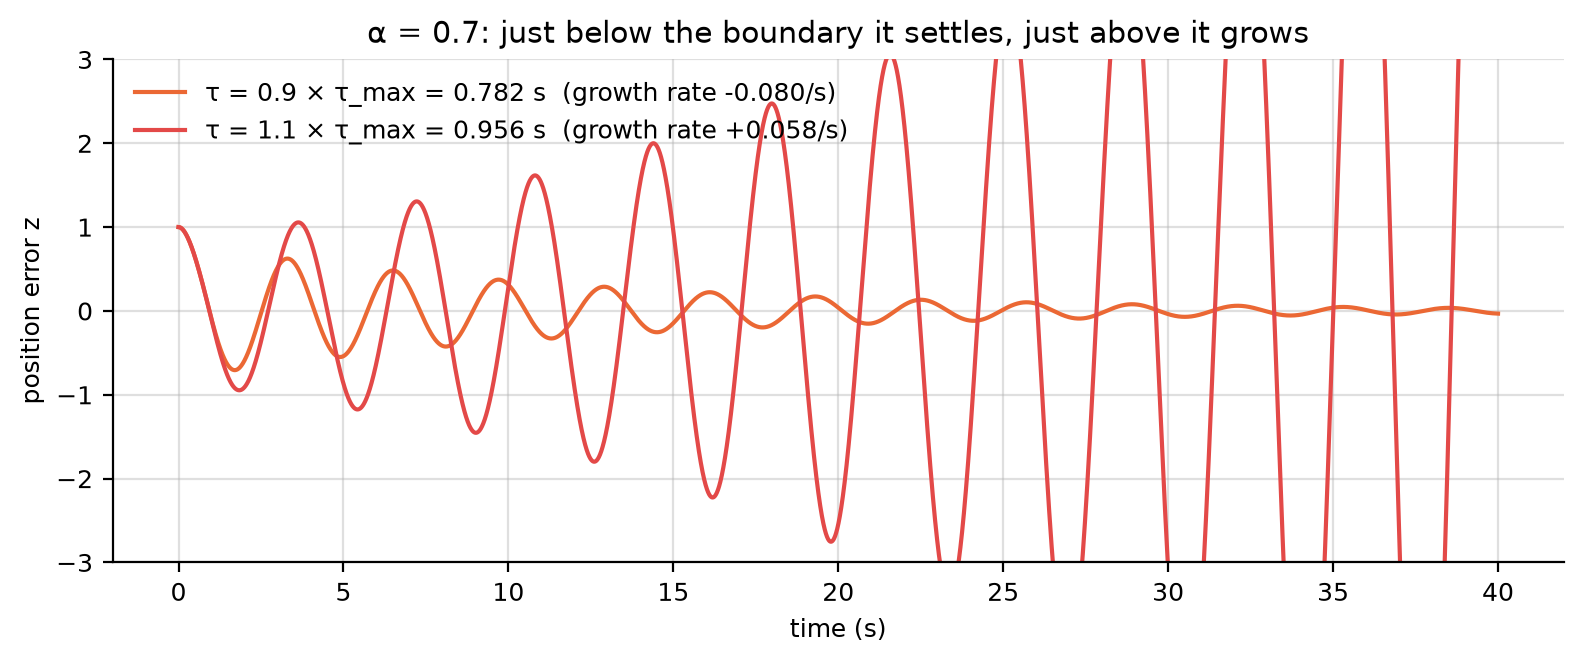
\includegraphics[width=0.85\textwidth]{16_s7_dde_either_side.png}
\caption{Direct simulation of the DDE at $\alpha = 0.7$, just below and
just above the formula's $\tau_{\max} = 0.869$\,s \ptwo{7.2}.}
\label{fig:dde}
\end{figure}

Finally, \emph{bisection} finds the boundary from simulation alone: keep
halving the interval between a delay that decays and one that grows
until it is narrower than $10^{-5}$\,s. Table~\ref{tab:sim} compares the
result with the formula; they agree to a few parts in a million.

\begin{table}[H]
\centering\small
\begin{tabular}{@{}cccc@{}}
\toprule
$\alpha$ & formula (s) & simulation (s) & relative error \\
\midrule
0.6 & 1.140974 & 1.140974 & $1.4\times10^{-7}$ \\
0.8 & 0.711439 & 0.711440 & $1.0\times10^{-6}$ \\
1.0 & 0.529029 & 0.529031 & $4.0\times10^{-6}$ \\
\bottomrule
\end{tabular}
\caption{Formula against bisection on the simulated DDE
(\code{tau\_max\_formula\_vs\_simulation.csv}).}
\label{tab:sim}
\end{table}

\begin{figure}[H]
\centering
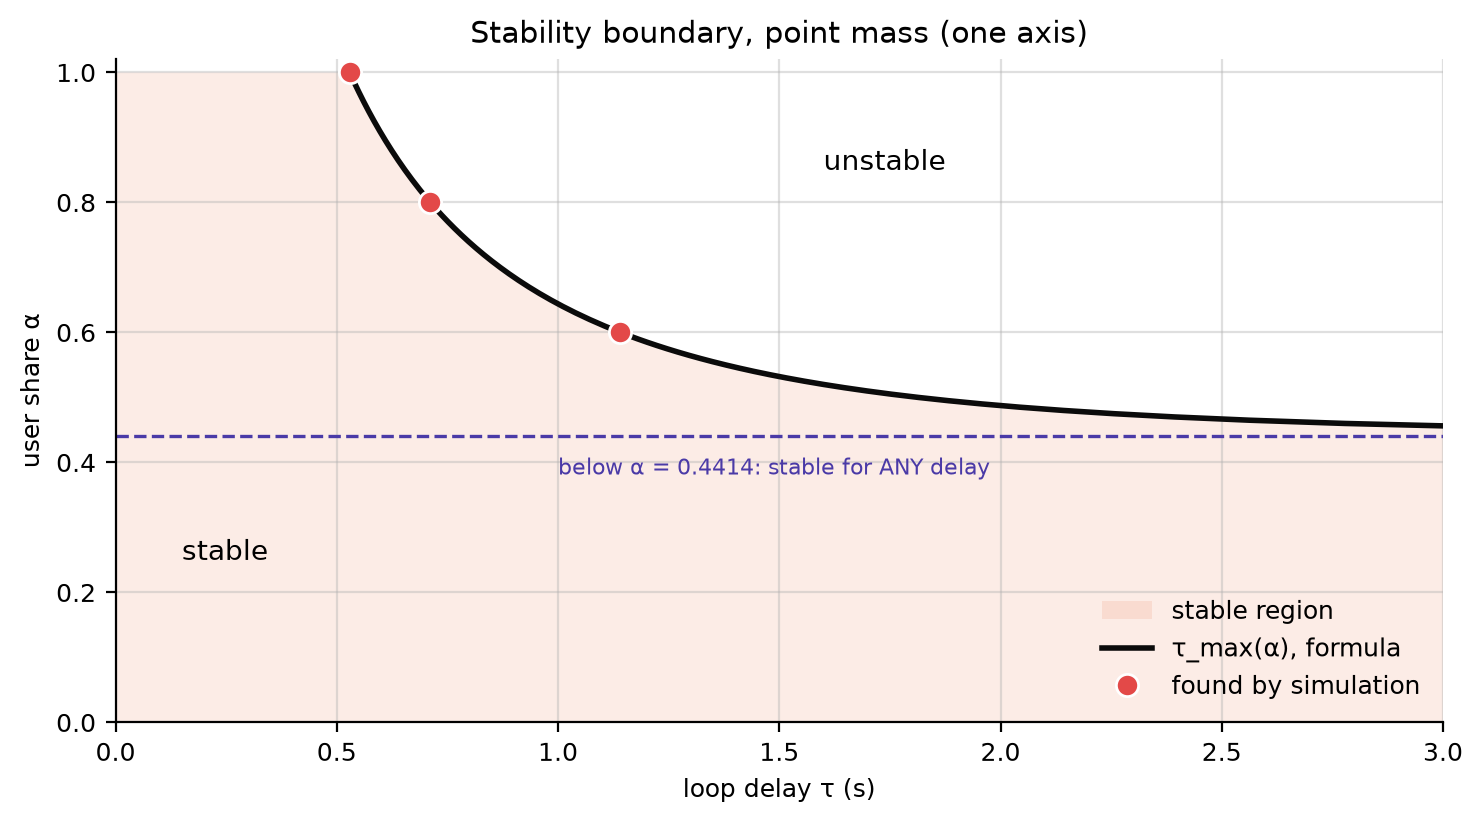
\includegraphics[width=0.8\textwidth]{17_s7_stability_boundary.png}
\caption{The result: the stability boundary $\tau_{\max}(\alpha)$ from
\eqref{eq:taumax} (curve), the simulation results of
Table~\ref{tab:sim} (dots), and the delay-independent region below
$\alpha = 0.4414$ (Section~\ref{sec:alphastar}).}
\label{fig:boundary}
\end{figure}

% =====================================================================
\section{Limitations and future work}
\label{sec:limits}

\subsection{Limitations}
\begin{itemize}\setlength{\itemsep}{2pt}
\item \textbf{Linear, single-axis model.} The exact result holds for the
damped double integrator. The simulated wheelchair is nonlinear,
nonholonomic and saturated; the heading-loop reduction
(Section~\ref{sec:heading}) analyses only the turn rate $\omega$, not
the speed $v$.
\item \textbf{Constant share $\alpha$.} The boundary is computed with
$\alpha$ frozen. The adaptive rule varies $\alpha$ over time (slowly, by
design), and a loop that is stable for every frozen $\alpha$ is not
guaranteed to be stable when $\alpha$ changes. The boundary is a guide
for the adaptive rule, not a proof.
\item \textbf{Constant delay.} The analysis assumes one fixed delay
$\tau$. In the simulator the decoder issues a decision every 2\,s and
holds it, so the age of the command varies between decisions; this is a
time-varying delay with a sample-and-hold, not a constant one.
\item \textbf{Stand-in controllers.} The autopilot is represented by LQR
and the user by a linear PD law; in the simulator the autopilot is a
planner (DWA) and the delay enters the user's target rather than the
feedback.
\item \textbf{Saturation ignored.} Command and acceleration limits are
not part of the linear analysis.
\end{itemize}

\subsection{Future work}
\begin{itemize}\setlength{\itemsep}{2pt}
\item Analyse the delay where it actually sits in the simulator (on the
reference) and include the 2\,s sample-and-hold, for example with a
discrete-time model.
\item Extend the analysis to a time-varying $\alpha(t)$, for example with
Lyapunov--Krasovskii methods, which handle time-varying delays and
gains.
\item Linearise the full unicycle about a reference path, including the
speed loop and its coupling to heading, and repeat the boundary
calculation for that model.
\item Account for saturation, for example with absolute-stability
(circle or Popov) criteria.
\item Compare the predicted boundary with the full wheelchair simulator
by deliberately moving the delay into the feedback path.
\end{itemize}

% =====================================================================
\section*{Summary}
\begin{itemize}\setlength{\itemsep}{1pt}
\item LQR gains: $K_1 = 3.162278$, $K_2 = 1.885231$, from the Riccati
equation solved by hand \eqref{eq:lqr}.
\item The delay only rotates the user's term, so it cancels from the
crossing condition, leaving the quadratic \eqref{eq:quad};
$\tau_{\max}(\alpha)$ follows in closed form \eqref{eq:taumax}.
\item User alone: $\tau_{\max}(1) = 0.529$\,s, equal to the classical
delay margin.
\item Stable for any delay below $\alpha = 0.4414$; the simple bound
$\alpha^* = 0.4415$ is slightly too high because $b(\alpha^*) < 0$.
\item Heading loop: $\alpha^* = 0.6126$ (exact), $\tau_{\max}(1) = 0.647$\,s.
\item Checks: \code{control} library ($2.2\times10^{-16}$\,s), direct
DDE simulation ($\le 4\times10^{-6}$ relative); Pad\'e over-estimates by
0.33--2.55\%.
\end{itemize}
These are the values reported in Table~6 of the main report,
\code{report.pdf}.

\begin{thebibliography}{9}\small
\bibitem{cooke1986zeroes}
K.~L. Cooke and P.~van~den Driessche.
On zeroes of some transcendental equations.
\emph{Funkcialaj Ekvacioj}, 29(1):77--90, 1986.

\bibitem{gu2003delay}
K.~Gu, V.~L. Kharitonov, and J.~Chen.
\emph{Stability of Time-Delay Systems}.
Birkh\"auser, Boston, 2003.
\end{thebibliography}

\end{document}
